\section{Algorithmic Optimizations} \label{sec:algopti}
In this section we will review algorithmic optimization techniques to reduce computational complexity of convolutions, which are a costly operation. According to \cite{shawahna_fpga-based_2019}, 90\% of computation time in \acrshort{cnn} are consummed by the convolution operation.
%
%
\subsection{\acrfull{gemm}}
%
%
It is a common way to process \acrshort{cnn} on \acrshort{cpu} and \acrshort{gpu}. We convert the convolution as a matrix-vector multiplication.  The process of a convolution layer can be observed on Figure \ref{fig:gemm}.
However, this approach is not suggested for \acrshort{fpga}: \cite{sze_efficient_2017, zhu_efficient_2020} point out that the \acrshort{fm}s have to be copied multiple times when flattened to a vector. It leads to a huge memory footprint and either ineffiency in storage or complex memory management access patterns.
\begin{figure}
    \centering
    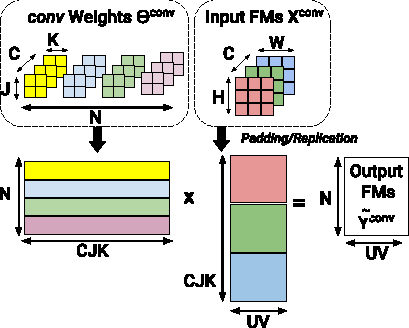
\includegraphics[width=0.5\textwidth]{Images/gemm.pdf}
    \caption{\acrshort{gemm} base processing on convolution layer \cite{abdelouahab_accelerating_2018}}
    \label{fig:gemm}
\end{figure}
%
%
\subsection{Fast algorithms for convolution}
The \acrshort{gemm} approach does not reduce the number of operations. In this section, we explore fast algorithms that aim at reducing the arithmetic complexity of the convolution operation, in particular Winograd and \acrfull{fft}. The fast convolution algorithms produces a tile of output instead of a single pixel. The fast convolutions can also be described by a common formula seen on equation \ref{eq:comform} where $\odot$ is the element-wise multiplication, $FM_O, FM_I$ the output and input \acrshort{fm}
\begin{equation}
FM_O = \boldsymbol{Inverse\_Transform} [ \ \boldsymbol{Transform}(FM_I) \odot \boldsymbol{Transform}(Kernel) ]
\label{eq:comform}
\end{equation}
%
\subsubsection{Winograd-based convolution}
%
The Winograd minimal filter algorithm is first introduced by \cite{winograd_arithmetic_1980}. In Winograd filtering, data is processed by blocs referred as \textit{tiles}, as following:
\begin{itemize}
    \item An input \acrshort{fm} tile $g$ of size $(N_{ix} \times N_{iy})$ is pre-processed: $\boldsymbol{Transform}(FM_I) = \boldsymbol{G^{T}} FM_I \boldsymbol{G} $
    \item In a same way, $Kernel$, of size $(K_x \times K_y)$ is also transformed: $\boldsymbol{Transform}(Kernel) = \boldsymbol{B^{T}} Kernel \boldsymbol{B}$.
    \item The inverse transformation function is then applied to obtain the output tile: $\boldsymbol{Inverse\_Transform}(E) = \boldsymbol{A^{T}} E \boldsymbol{G}$, where $E$ is the result of the element-wise multiplication of the two transformed tile.
\end{itemize}
The output tile $FM_O$ of the Winograd Filtering algorithm, denoted $F(N_{ix} \times N_{iy}, K_x \times K_y)$ is computed using equation \ref{eqn:winograd}. The advantage of using the Winograd-based convolution is that the transformation matrix $\boldsymbol{G}, \boldsymbol{B}, \boldsymbol{A}$ can be computed off-line using the Winograd Algorithm \cite{winograd_arithmetic_1980} once $N_{ix}, N_{iy}, K_x, K_y)$ are fixed.
\begin{equation}
\label{eqn:winograd}
FM_O = \boldsymbol{A^{T}} [ \ \boldsymbol{G^{T}} FM_I \boldsymbol{G} \odot \boldsymbol{B^{T}} Kernel \boldsymbol{B} \ ] \boldsymbol{A}
\end{equation}
%
\subsubsection{\acrshort{fft}-based convolution}
%
The \acrshort{fft}, introduced by \textcite{cooley_algorithm_1965}, is an algorithm to transform the tile into the frequency domain. It can be integrated into the convolution to reduce the number of operation, where:
\begin{itemize}
    \item $\boldsymbol{Transform} = FFT$
    \item $\boldsymbol{Inverse\_Transform} = IFFT$
\end{itemize}
%
\subsubsection{Comparaison}
Winograd-based convolution seems to be a prefered way to perform fast convolution. This is explained by three reasons: \textcite{lavin_fast_2015} demonstrated that Winograd convolution is efficient when the kernel is small ($K_* \leq 3$) and the stride is equal to 1; second \acrshort{fft}-based convolution are only feasible when the kernel is large \cite{ahmad_towards_2019, chitsaz_acceleration_2020}; third, current \acrshort{cnn} trends prior the utilisation of small kernel \cite{liang_evaluating_2020, sandler_mobilenetv2_2019}. \newline
Moreover, FPGA implementations of Winograd algorithm have produced good results. For example, \cite{aydonat_opencl_2017, liang_evaluating_2020} utilized Winograd transform and haved reduced their computational complexity by around 50\% but Winograd algorithm also increases also increases the bandwith utilization \cite{xiao_exploring_2017}. However, \textcite{zeng_optimizing_nodate, chitsaz_acceleration_2020, liang_evaluating_2020} have made works on optimizing the frequency-domain convolution with small filter by using Overlap-and-Add technique \cite{w_smith_scientist_1997} to lower the number of operations and increase the data parallelism. Still, according to \textcite{liang_evaluating_2020, podili_fast_2017}, \acrshort{fft} requires more memory, bandwith, and logic resources (more additions and multiplications) than Winograd.
